\chapter{Prozess Architekturplanung}
Aufbauend auf den im Anforderungsprozess ermittelten Attribute, kann nun mit der Architekturplanung begonnen werden.

\section{Erstellen der Minimalen Architektur}
Das Kontext Diagramm, welches im Anforderungsprozess erstellt worden ist, zeigt das System mit allen AkteurInnen und Nachbarsystemen. Aufbauend darauf kann nun die minimale Architektur erstellt werden, welche sich aus dem System und den Nachbarsystemen ableitet.

\begin{figure}[H]
    \centering
    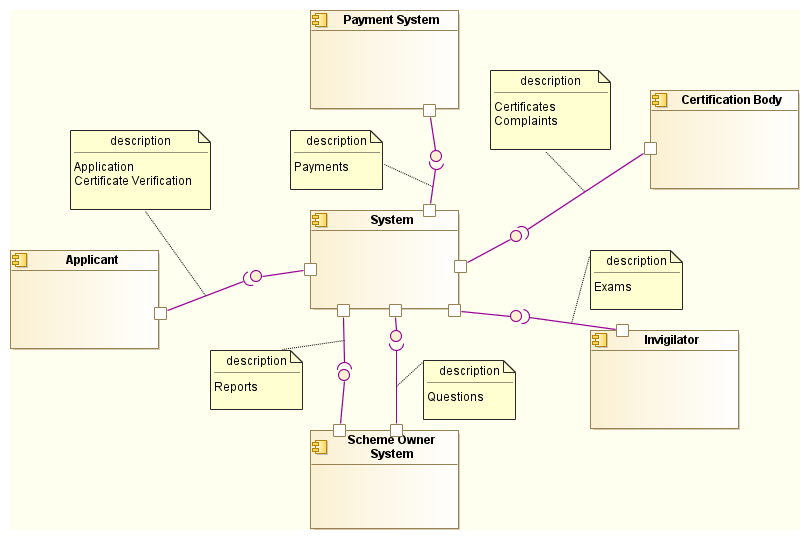
\includegraphics[scale=0.5]{uml/context.png}
    \caption{Das Kontext Diagramm liefert die Ausgangsbasis für die Architektur}
\end{figure}

Zuerst werden alle Datenflussnotizen entfernt. Danach werden alle Komponenten entfernt, welche kein eigenes System darstellen. In diesem Falle werden folgende Komponenten entfernt:

\begin{itemize}
  \item Applicant
  \item Certification Body
  \item Invigilator
\end{itemize}

Dies führt zu folgender Minimalarchitektur:

\begin{figure}[H]
    \centering
    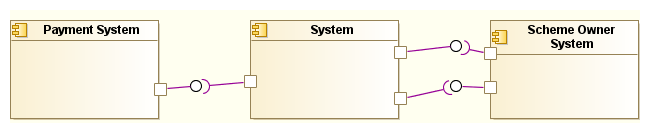
\includegraphics[scale=0.7]{uml/minimalarch.png}
    \caption{Minimale Architektur}
\end{figure}

Für die Nachbarsysteme wird keine Architektur erstellt, jedoch beinflussen sie die Schnittstellen des Systemes und sind deswegen wichtig für den weiteren Prozes. Sie werden in die Architektur einbezogen und in die niedrigste Vertrautheitsebene eingeteilt.

\section{Erstellen der Datenminimalarchitektur}
Auf Basis der Vertrautheitskategorien der Daten wird das System der vorher erstellte Minimalarchitektur in ebenso viele Teilsysteme unterteilt. Die Aktivitätsdiagramme werden an die neue Architektur angepasst: Für jedes Untersystem wird in den Diagrammen eine eigene Swimlane erstellt. Die involvierten AkteurInnen sind wenn möglich als eigene Swimlane modelliert, spielen in dieser Phase aber noch keine wichtige Rolle zur Gliederung des Systemes.

\begin{figure}[H]
    \centering
    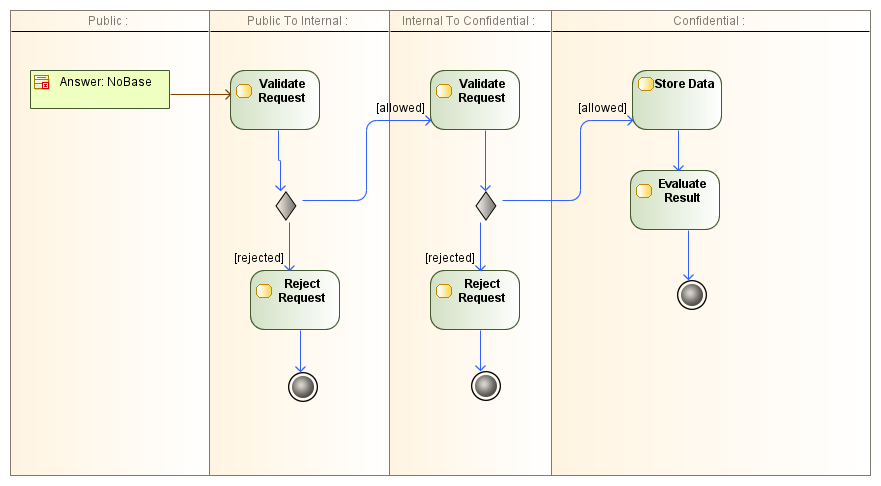
\includegraphics[scale=0.5]{uml/takeexamactivity1.png}
    \caption{Die Antworten werden nach der Prüfung an den Certification Body übermittelt. Der Request wird dann durch zwei Gateways zum finalen System geleitet.}
\end{figure}

Wechselt der Kontrollfluss eine Swimlane, heißt dies, dass eine Verbindung zwischen den beiden sonst abgeschotteten Systemen benötitgt wird. Dieses Verbindung wird als eigenes System modelliert und wird als Gateway bezeichnet. Die Aufgabe dieses Gateways ist es, folgende Attribute der Anfrage zu überprüfen und die Anfrage gegebenenfalls zu verwerfen oder weiterzuleiten:

\begin{itemize}
  \item Von welchem System kommt die Anfrage?
  \item Welches System ist das Ziel der Anfrage?
  \item Welche Schnittstelle dieses Systems ist das Ziel der Anfrage?
  \item Gibt es eine Regel die diese Anfrage explizit erlaubt?
\end{itemize}

\begin{figure}[H]
    \centering
    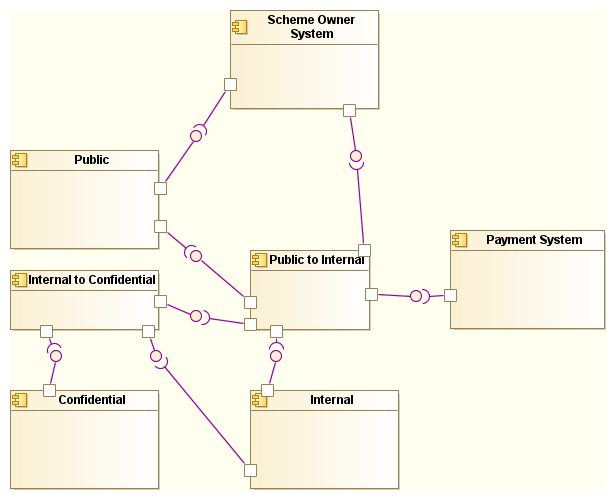
\includegraphics[scale=0.7]{uml/dataarch.png}
    \caption{Aufteilung der Komponenten in Datenbereiche}
\end{figure}

Wichtig ist hier, dass keine Gateways unterschiedlicher Vertrautheitsebenen übersprungen werden. Zeigt ein Aktivitäts Diagramm zB. einen Zugriff von Ebene 1 auf Ebene 3 muss dieser Zugriff sowohl durch den Gateway der Ebene 2 geleitet werden, als auch durch den Gateway der Ebene 3. Dies verhindert, dass besonders schützenswerte Systeme direkt an Systeme mit einem weitaus niedrigeren Vertrautheitsgrad angeschlossen werden und so dessen Gateway zum Single Point of Failure wird. Dies gilt in beide Richtungen.

Da bei der Erstellung des Systems alle Schnittstellen und Systeme bekannt sind, können diese Regeln fest im Gateway verankert werden. Weil diese Gateways unabhängig voneinander agieren, können sie durch das Hinzufügen eines Load Balancers beliebig vervielfacht werden, was sowohl die Ausfallsicherheit als auch die Skalierbarkeit erhöht. Das ist wichtig, weil sie als einzige Verbindung zwischen den Systemen zu einer Art Flaschenhals werden.


\section{Einbinden der AkteurInnen}
Nachdem die Datenminimalarchitektur steht, können nun die AkteurInnen des Systems in die Aufgliederung des Systemes mit einbezogen werden. Hierfür müssen nun die Objektflüsse und die AkteurInnen des Systems für jeden Usecase betrachtet werden, welche aus den vorher bereits erstellten Aktivitätsdiagramm ersichtlich sind.

Zuerst wird das erste Untersystem, in diesem Falle das Public System, betrachtet. Alle Objektflüsse durch das System und die AkteurInnen, welche mit ihren Swimlanes angrenzen, sind in die Aktivitäten des Systems involviert. Jede Involvierung eines Akteures in ein System erfordert einen Zugang zu diesem System.

Jeder dieser Akteure muss mit den minimal möglichen Rechten für dieses System ausgestattet werden, um seine Aufgaben zu erfüllen. Dies vermeidet nicht nur Fehler sondern reduziert auch den Schaden, welcher ein potentieller Angriff dieses Akteurs/dieser Akteurin anrichten kann \cite[1. A]{leastpriv}.

Da ein System komplex ist \cite[S. 7]{softarch}, und diese Sicherheitsattribute nach Änderungen am System immer wieder überprüft werden müssen, stellt jeder zusätzliche Zugriff eines Akteures nicht nur ein Sicherheitsrisiko dar, sondern erhöht auch den Test- und damit den Wartungsaufwand. Idealerweise wird daher jedem/jeder AkteurIn ein eigenes, für sich abgekapseltes System zur Verfügung gestellt, was jedoch meist aufgrund Kosten der zusätzlichen Systeme keine Option dar stellt.

Deswegen wird nun anhand der Aktivitäts Diagramme der Usecases und in der Anforderungsanalyse ermittelten Schadenstabelle des unerlaubten Datenzugriffs eine Aufspaltung in mehrere Systeme vorgenommen, falls die Schadenskosten die eines neuen Systemes überschreiten.

Im Falle des Beispielprojektes wird zB. für die stark vereinfachten Aktivitäts Diagramme in Abbildung \ref{fig:actorarch} ermittelt, dass die möglichen Schadenskosten im Falle, dass der Anwärter (Applicant) Zugriff auf die Prüfungsantworten (Answer) bekommt, die eines eigenen Systems überschreiten. Deswegen wird der Usecase aus dem Public System in eigenes System entkoppelt.

\begin{figure}[H]
    \centering
    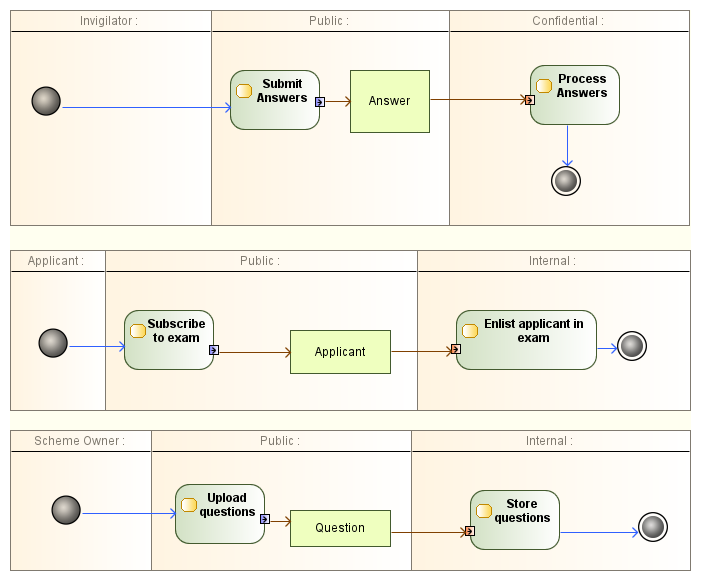
\includegraphics[scale=0.6]{uml/actorarch.png}
    \caption{Vereinfachte Gegenüberstellung von Aktivitätsdiagramme für das Public System}
    \label{fig:actorarch}
\end{figure}

Diese Analyse wird für alle verbleibenden Systeme durchgeführt, bis alle Systeme aufgespalten sind. Für den Fall, dass bei der Aufspaltung zu viele Systeme entstanden sind, werden nun in einem weiteren Schritt diverse Teilsysteme wieder zusammen gelegt, solange deren Schadenskosten nicht die Systemkosten überschreiten. Dies wird solange durchgeführt, bis eine minimale Anzahl an Systemen verfügbar ist.

Im Falle des Beispielprojektes führt dies schlussendlich zu folgender Systemaufspaltung:

\begin{figure}[H]
    \centering
    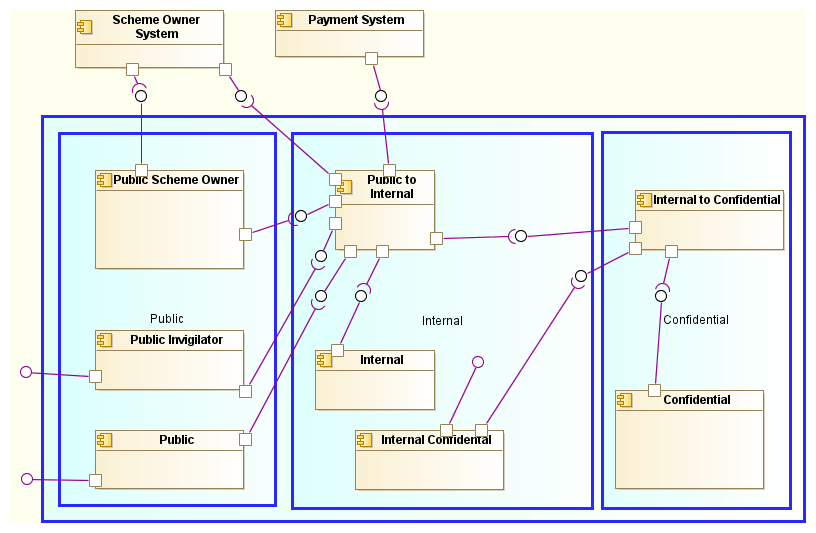
\includegraphics[scale=0.6]{uml/vision4.png}
    \caption{Architektur nach der Aufspaltung }
\end{figure}

TODO: Architektur überprüfen

\section{Modellieren der Komponenten Interfaces (Klassen Diagramm)}
Aufzeigen dass zb das interne System user anlegen können muss mit methoden im klassendiagramm

\section{Analyse der nicht funktionalen Attribute}
Auf Basis von dokumentierten Szenarien können nun nicht funktionale Attribute gemessen werden und Hinweise kritische/wichtige Komponenten gegeben werden. Kostengegenüberstellung können auch eigene Systeme rechtfertigen/entfernen

\subsection{Reliability}
Single Point of Failure Analyse (Matrix Komponente x Usecase), Erklären wie man auf Matrix kommt (Aktivitätsdiagramm), Ausfallskosten (inkl. Wachstumsszenarien)

Einfache Methode zur schätzung der Ausfallkosten, aufzeigen wie durch Reduzieren der Ausfallswahrscheinlichkeit Kosten sinken aber auch Investitionskosten verursachen. Wachstumsszenarien auch einbeziehen in die Rechnung
\subsection{Usability}
In diesem Teil des Prozesses nicht wichtig, da noch keine Implementierung vorhanden.

\subsection{Efficiency}
Efficiency kann pro usecase gemessen werden, zb für antwortzeiten indem man zb die swimlanewechsel der Aktivitätsdiagramme zählt und mit einer konstanten multipliziert (geschätzte Netzwerkgeschwindigkeit). Ansonsten ist es durch die fehlende Implementation nicht möglich die Geschwindigkeit oder den Arbeitsspeicherverbrauch zu messen.

\subsection{Maintainability}
Auslesbar aus der Usecase Matrix, als Summe aller subsysteme,

\subsection{Portability}
In diesem Teil des Prozesses nicht wichtig, da noch keine Implementierung vorhanden.
